\subsection{Theorem}
\begin{namedframe}{Theorem}
	\vspace{-2ex}
	\begin{theorem}[``Star Trek'' Theorem]
		The central angle \alert{subtended} by any arc is twice any of the inscribed angles on that arc.

		This means that in the diagram, $\angle AOB = 2 \angle ACB$.
	\end{theorem}
	\pause
	\centering
	\begin{columns}
		\begin{column}{0.5\textwidth}
			\centering
			\begin{tikzpicture}[scale=0.4]
				\coordinate [label=left:$O$](O) at (0,0);
				\coordinate [label=below left:$A$](A) at (-3,-4);
				\coordinate [label=below right:$B$](B) at (4,-3);
				\coordinate [label=above left:$C$](C) at (-1,4.89897948557);
				\coordinate [label=below:$L$](L) at (0.5,-2.44948974278);

				\draw (O) circle (5);
				\draw (A) -- (O) -- (B) -- (C) -- cycle;
				\draw [dashed] (C) -- (L);

				\only<6>{\pic [draw, "$\alpha$", angle eccentricity=1.25, angle radius=7mm] {angle = O--A--C};}
				\only<6>{\pic [draw, "$\alpha$", angle eccentricity=1.25, angle radius=7mm] {angle = A--C--O};}

				\only<7>{\pic [draw, "$\beta$", angle eccentricity=1.25, angle radius=1cm] {angle = O--C--B};}
				\only<7>{\pic [draw, "$\beta$", angle eccentricity=1.25, angle radius=1cm] {angle = C--B--O};}
			\end{tikzpicture}
		\end{column}
		\begin{column}{0.5\textwidth}
			Here, $\angle AOB$ is \alert{subtended} by the \alert{minor arc} from $A$ to $B$.
			\sep
			A \alert{minor arc} is the smaller of the two arcs that can be formed by two points on a circle.
			\sep
			Also, note that $\triangle OAC$ and $\triangle OBC$ are isosceles.
			\pause
			This is because $OA$, $OB$, and $OC$ are all radii.
			\pause
			So, $\angle OAC = \angle OCA$ \pause and $\angle OCB = \angle OBC$.
		\end{column}
	\end{columns}
\end{namedframe}
\subsubsection{Proof}
\begin{namedframe}{Proof of the Star Trek Theorem}
	\footnotesize
	\begin{proof}[Proof that $\angle AOB = 2 \angle ACB$]
		\begin{wrapfigure}[0]{r}{0pt}
			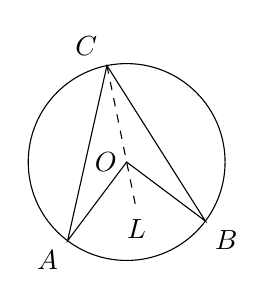
\begin{tikzpicture}[scale=0.25]
				\coordinate [label=left:$O$](O) at (0,0);
				\coordinate [label=below left:$A$](A) at (-3,-4);
				\coordinate [label=below right:$B$](B) at (4,-3);
				\coordinate [label=above left:$C$](C) at (-1,4.89897948557);
				\coordinate [label=below:$L$](L) at (0.5,-2.44948974278);

				\draw (O) circle (5);
				\draw (A) -- (O) -- (B) -- (C) -- cycle;
				\draw [dashed] (C) -- (L);
			\end{tikzpicture}
		\end{wrapfigure}
		We know that $\angle OAC = \angle OCA$.
		\pause
		So: $2\angle OCA + \angle AOC = \SI{180}{\degree}$.
		\sep
		And we know that $\angle AOC + \angle AOL = \SI{180}{\degree}$.
		\pause
		\begin{align*}
			2\angle OCA + \angle AOC &= \angle AOC + \angle AOL\\
			\angle OCA &= \frac{1}{2}\angle AOL
		\end{align*}
		\pause
		And similarly for $\triangle OBC$: $\angle OCB = \frac{1}{2} \angle BOL$.
		\pause
		\begin{align*}
			\uncover<+->{\angle ACB &= \angle OCA + \angle OCB\\}
			\uncover<+->{\angle ACB &= \frac{1}{2}\angle AOL + \frac{1}{2}\angle BOL\\}
			\uncover<+->{\angle ACB &= \frac{1}{2}(\angle AOL + \frac{1}{2}\angle BOL)\\}
			\uncover<+->{2\angle ABC &= \angle AOB}
		\end{align*}
		\uncover<+->{\qedhere}
	\end{proof}
\end{namedframe}
